% Modelo de relatório no estilo artigo em duas colunas
\documentclass[twocolumn]{article}
\usepackage[utf8]{inputenc}
\usepackage{amsmath}
\usepackage{subcaption}
\usepackage{mathtools}
\usepackage{graphicx}
\usepackage{color}
\usepackage{authblk}
\usepackage{lmodern}
% \usepackage[colorlinks,citecolor=black,urlcolor=black,bookmarks=false,hypertexnames=true]{hyperref}
\usepackage[margin=0.9in]{geometry}
\usepackage{pdfpages}
\usepackage{fancyhdr}
\usepackage[utf8]{inputenc}
\usepackage{hyperref}

\usepackage[sorting=none,style=numeric]{biblatex}
\addbibresource{refs.bib}
\usepackage[justification=centering]{caption}
\usepackage{makecell}
\usepackage{booktabs}
\usepackage{hhline}
\usepackage{amsmath}
\usepackage{amssymb}
\usepackage{soul}
\usepackage{gensymb}
\usepackage{listings}
\usepackage{lstlinebgrd}

\setlength\parindent{0pt}


\newcommand{\myname}{Nishant Aswani}
\newcommand{\mynetid}{nsa325}
\newcommand{\myemail}{nsa325@nyu.edu}
\newcommand{\myhwtype}{Final Project Report}
\newcommand{\myhwnum}{}
\newcommand{\mycoursenumber}{ENGR-UH 3511}
\newcommand{\myclassname}{Computer Organization and Architecture }
\newcommand{\myassignmenttitle}{Compiling a LSTM Neural Network for Various ISAs using the Glow and LLC Compilers}
\newcommand{\myinstructor}{Mihalis Maniatakos}

\newcommand{\cc}[1]{\texttt{#1}}

\lstset{
  basicstyle=\ttfamily,
  escapeinside=||,
  commentstyle=\color{red},
  keywordstyle=\color{blue}
}

% Tamanho das margens:
% \geometry{
% 	a4paper,
% 	total={170mm,257mm},
% 	left=30mm,
% 	top=20mm,
% }
%%%%%%%%%%%%%%%%%%%%%%%%%%%%%%%%%%%%%%%%%
% Bibliografia estilo ABNT. Se não tiver instalado, comente a linha abaixo.
% \usepackage[alf, abnt-etal-list=0, abnt-emphasize=bf,abnt-last-names=bibtex, abnt-etal-text=it, abnt-etal-cite=2]{abntex2cite}
%%%%%%%%%%%%%%%%%%%%%%%%%%%%%%%%%%%%%%%%%

% Dados de identificação
\title{\myassignmenttitle}
\author{\myname, \myemail}
\affil{\myclassname (\mycoursenumber), Professor \myinstructor}
\date{}

\begin{document}
%%%%%%%%%%%%%%%%%%%%%%%%%%%%%%%%%%%%%%%%%%%%%%%% COVER PAGE %%%%%%%%%%%%%%%%%%%%%%%%%%%%%%%%%%%%%%%%%%%%%%%%%%%%
\onecolumn
\pagestyle{fancy}
\fancyhf{}
\renewcommand{\headrulewidth}{0pt}
\rhead{\textbf{Division of Engineering}}
\lhead{\textbf{NYU Abu Dhabi}}

\begin{center}
  
\includegraphics[scale=0.15]{etc/NYUAD-alt-logo.jpg}
\end{center}

{\vspace{2.5em}}

\begin{center}
    \Huge{\textbf{\mycoursenumber}}\\
    {\vspace{0.5em}}
    \Huge{\textbf{\myclassname}}
\end{center}

{\vspace{10em}}

\begin{center}
  \begin{tabular}{|rp{5.0cm}lll|}
    \hline
    &  &  &  & \\
    &  &  &  & \\
    \Large{\textbf{Name:}} & \Large{\myname}
    
    \  &  &  & \\
    \Large{\textbf{Net ID:}} & \Large{\mynetid}
    
    \  &  &  & \\
    \Large{\textbf{Assignment Title:}} & \Large{\myhwtype \myhwnum}
    
    \
    
    \  &  &  & \\
    \hline
  \end{tabular}
\end{center}

\

{\newpage}
%%%%%%%%%%%%%%%%%%%%%%%%%%%%%%%%%%%%%%%%%%%%%%%% COVER PAGE %%%%%%%%%%%%%%%%%%%%%%%%%%%%%%%%%%%%%%%%%%%%%%%%%%%%

\maketitle        

% Resumo de no máximo 200 palavras
% \begin{abstract}
% Este documento orienta a descrição das atividades práticas desenvolvidas em laboratório. São usados como exemplo conceitos da Aula 01 de Acionamentos Elétricos sobre partida direta de motor de indução trifásico. Nesta atividade, um motor é acionado com conexões estrela e triângulo a vazio. As correntes nominais e de partida são medidas com amperímetro analógico e comparadas entre si. Nota-se que, mesmo sem carga, as corrente em estrela são maiores. 
% \end{abstract}

\section{Introduction}

With the advent of machine learning (ML) techniques being applied for forecasting and vision, along with increasing abilities to gather data, rose the need for specific hardware. Traditional CPUs are unable to efficiently exploit the parallelism in the operations carried out in neural networks \cite{sze2017hardware}. Application-specific integration circuits (ASICs) for machine learning, on the other hand, are designed specifically to exploit the repetitive and predictable operations of a neural network. These specific architectures. Some of the main principles of domain-specific architectures (DSAs) include "dedicated local memories, large numbers of arithmetic units, [and] simple forms of parallelism", in the hopes of improving energy efficiency \cite{rotem2018glow}.\\

As a result, there is a need for compilers capable of optimizing deep neural networks (DNN) for execution on DSAs. Traditionally, frameworks "iterate over the nodes in the graph and execute them one by one" \cite{rotem2018glow}, leading to immense inefficiences. Compilers, such as Glow, take into account the entire network representation before making compilation decision, in hopes to improve efficiency regardless of hardware. \\

This project makes use of Glow to compile a bidirectional Long short-term memory (LSTM) model on various instruction set architectures (ISAs) in hopes to explore what typical ML operations look like as instructions as well as compare how relatively complex instructions are implemented in different architectures. 

\subsection{LSTM Model}

An LSTM is a form of recurrent neural network (RNN) designed as a solution to the "vanishing gradient" \cite{lstm} problem that RNN models face: context remembrance across long time lags "takes a prohibitive amount of time or does not work at all" \cite{lstm}. LSTMs have additional gates (forget, input, and output gates) compared to traditional RNNs which allow for them to be more robust and aid the model in deciding whether certain values should be used or not.\\

What makes an LSTM layer interesting is that it carries out more complex operations than the typical Dense layer of neurons, where a multiply and accumulate (MAC) is the dominant operation. Furthemore, looking at figure \ref{fig:lstm_cell}, we see within the gates (yellow containers) the use of sigmoid and tanh functions as activation functions for the LSTM cell. 

\newpage

\begingroup
    \centering
    \medskip
    %width=\columnwidth
    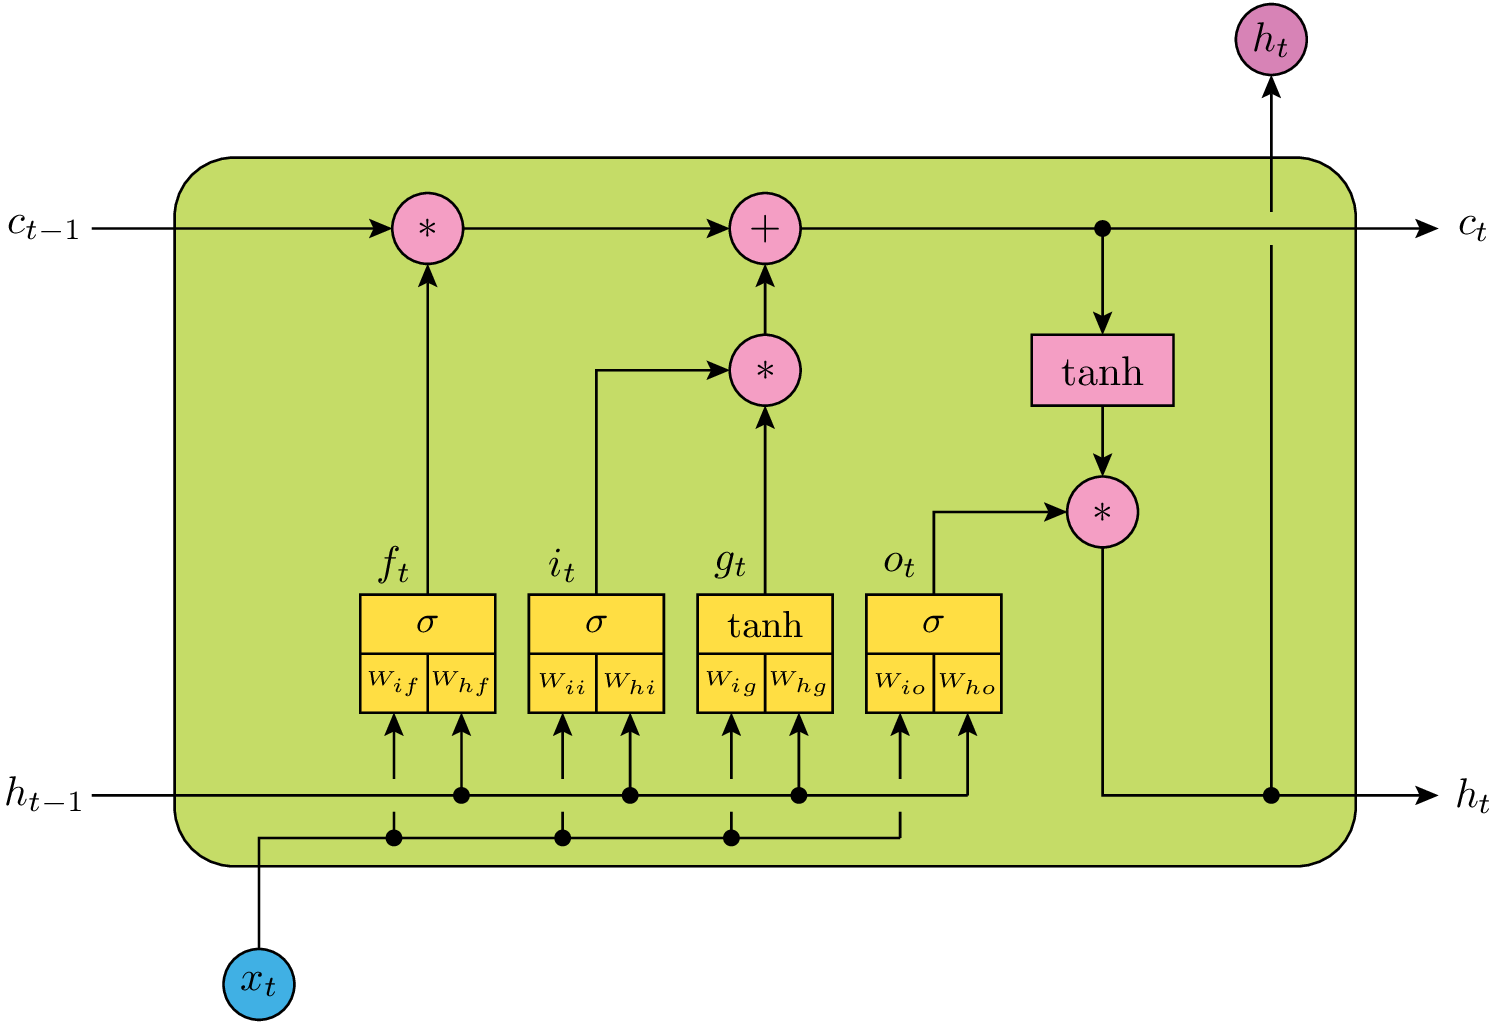
\includegraphics[width=0.4\columnwidth]{Lab-Tex/final/lstm.png}
    \captionof{figure}{Overview of a LSTM cell}
    \label{fig:lstm_cell}
\endgroup

\subsection{The \cc{tanh} function}

As implied above, the \cc{tanh} function is a popular motif in machine learning models. The purpose of an actiavtion function is to build a model to explain data which is non-linear. Without activation functions, neural networks would collapse to linear approximations. \\

In hardware, we must find a numerical method to compute such functions. One of the models for the \cc{tanh} function is shown here \cite{beebe1991accurate}: 

\begingroup
    \centering
    \medskip
    %width=\columnwidth
    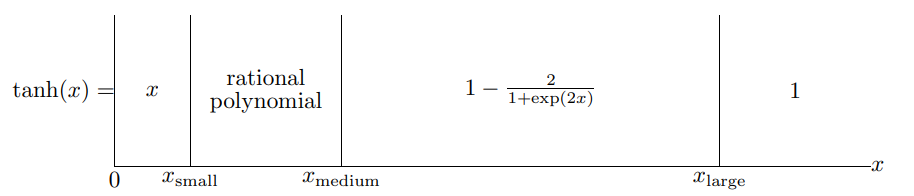
\includegraphics[width=0.7\columnwidth]{Lab-Tex/final/tanh.png}
    \captionof{figure}{Computing the tanh(x) function}
    \label{fig:tanh_funcs}
\endgroup




\section{Methodology}


The model used in this project, shown in Figure \ref{fig:netron_rep}, was obtained in the ONNX file format from a unit test of \href{https://github.com/microsoft/onnxruntime}{Microsoft's NN scoring engine} and visualized using \href{https://github.com/netron}{Netron}.\\

\begingroup
    \centering
    \medskip
    %width=\columnwidth
    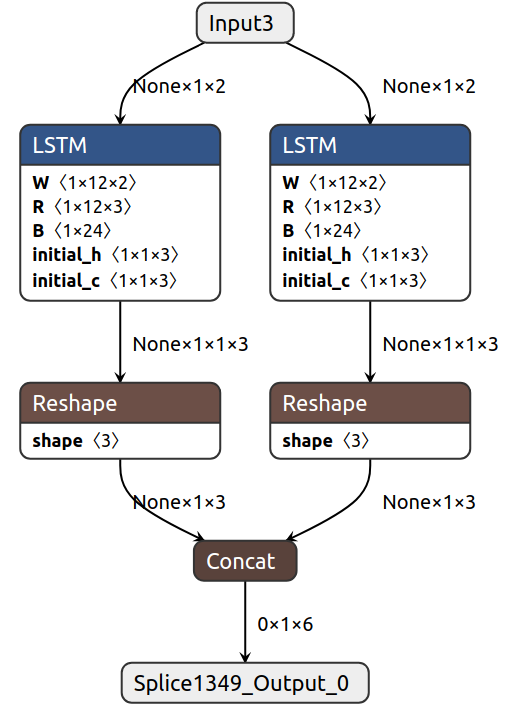
\includegraphics[width=0.3\columnwidth]{Lab-Tex/final/bilstm.png}
    \captionof{figure}{Visualizing the LSTM model}
    \label{fig:netron_rep}
    \medskip
\endgroup

The Glow compiler was built in release mode, which provided a \cc{model-compiler} binary capable of handling ONNX models as an input. \\

Using the following shell command, a \cc{'.s'} file containing assembly code was produced.:

\begin{lstlisting}[language=bash]
./model-compiler \ 
-model="../bilstm.onnx" -emit-bundle="../mips32_bundle" \ 
-backend=CPU -onnx-define-symbol=None,1 \ 
-llvm-compiler=/usr/bin/llc-8 -llvm-compiler-opt=-filetype=asm \
-target=mips -mcpu=mips32 \
-dump-graph-DAG=graph.dot -dump-llvm-ir > ir.txt
\end{lstlisting}
\medskip
 The \cc{-model} flag takes the path of the ONNX model, \cc{-emit-bundle} is the output directory. The \cc{-llvm-compiler} flag accepts an external compiler (in place of the default llvm compiler), for which the filetype was set to \cc{asm} to obtain assembly code instead of machine code. The \cc{-target=mips -mcpu=mips32} flags tell the \cc{llc} compiler which architecture to build for. Finally, the \cc{-dump} flags output the graph representation of the network and the low-level intermediate representation (IR), respectively. \\
 
 Figure \ref{fig:graph_rep} shows a slice of the the graph representation of the neural network. Towards the middle we see the activation functions in their own nodes. Hence, as part of the exploration, it was sought to discover how actviation nodes were represented in the low-level IR and assembly language. 

 \begingroup
    \centering
    \medskip
    %width=\columnwidth
    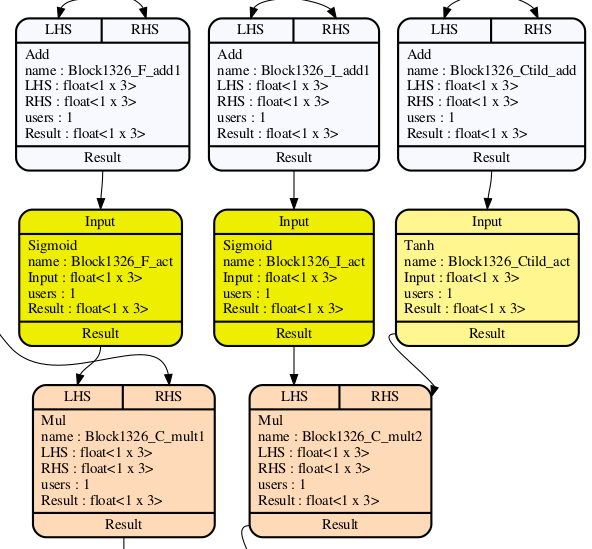
\includegraphics[width=0.5\columnwidth]{Lab-Tex/final/graph.png}
    \captionof{figure}{Graph representation using Glow}
    \label{fig:graph_rep}
    \medskip
\endgroup

 \section{Results and Discussion}
 
 \subsection{Intermediate Representation}
 
 Taking a look at the intermediate representation, multiple loops were found defined as \cc{stacked kernels}. Glow "stacks operators and performs a few data-parallel operators one after the other on the same memory location,"\cite{rotem2018glow} an optimization that cannot allegedly done by a traditional LLVM compiler.\\ 

The loop below represents the right hand size of Figure \ref{fig:graph_rep}:

\newpage

\begin{lstlisting}[basicstyle=\Footnotesize]
loop:                                             ; preds = %loop, %entry
  %3 = phi i64 [ 0, %entry ], [ %nextvar, %loop ]
  %4 = call float @libjit_element_add_kernel_f(i64 %3, float* %0, float* %1, float* null)
  %buffer.element.addr = getelementptr float, float* %0, i64 %3
  store float %4, float* %buffer.element.addr
  %5 = call float @libjit_tanh_kernel_f(i64 %3, float* %0, float* null, float* null)
  %buffer.element.addr1 = getelementptr float, float* %0, i64 %3
  store float %5, float* %buffer.element.addr1
  %6 = call float @libjit_element_mul_kernel_f(i64 %3, float* %2, float* %0, float* null)
  %buffer.element.addr2 = getelementptr float, float* %2, i64 %3
  store float %6, float* %buffer.element.addr2
  %nextvar = add nuw nsw i64 %3, 1
  %loopcond = icmp ult i64 %nextvar, 3
  br i1 %loopcond, label %loop, label %afterloop, !llvm.loop !6

afterloop:                                        ; preds = %loop
  ret void
}
\end{lstlisting}

We see that three operators \cc{add}, \cc{tanh}, and \cc{mul} have been combined into a single stack (see variables \%4, \%5, \%6). Furthermore, to represent the \cc{tanh} function there is a call to the \cc{libjit tanh kernel f} function. This tag will prove useful when parsing the assembly code for the different architectures.\\

The source files of the Glow compiler reveal how the \cc{tanh} function is implemented.

\begin{lstlisting}
DEFINE_DATA_PARALLEL_KERNEL(libjit_tanh_kernel_f, float,
                            1 - 2 / (expf(LHS[idx] * 2) + 1))
\end{lstlisting}

Unsurprisingly, Glow uses the most accurate way to compute the tanh function. This function is also seen in figure \ref{fig:tanh_funcs}.

\subsection{Compiling for MIPS32}
 
After compiling for the MIPS ISA, there were multiple \cc{jal} instructions such as these: 

\begin{lstlisting}
	jal	libjit_stacked_kernel.1_3_specialized
\end{lstlisting}

These labels were defined below and corresponded to assembly instructions of what was seen in the the intermediate representation. \textbf{For MIPS, the \cc{stacked kernel 1 and 3} were 60 lines of assembly instructions.} Since the label implies that this is a set of instructions for two stacked kernels, it was unclear which of the three \cc{expf} operations belonged to the \cc{tanh} function. Although, it is quite likely that the following chunk of instructions carries the \cc{tanh} operation: 

\begin{lstlisting}
        mul.s	$f0, $f1, $f0
	swc1	$f0, 0($16)
	lwc1	$f0, 4($17)
	lwc1	$f1, 4($18)
	add.s	$f0, $f1, $f0
	jal	expf
	add.s	$f12, $f0, $f0
	add.s	$f0, $f0, $f20
	div.s	$f0, $f21, $f0
	sub.s	$f0, $f20, $f0
\end{lstlisting}
\\
Interestingly, the MIPS assembly was littered with \cc{# 4-byte Folded Spill} comments generated by the compiler. Given that these comments were beside \cc{sw} instructions, it is likely that the 32 registers of the MIPS CPU were not enough for the computations carried out. Hence, the compiler is forced to interact with the memory, which is an expensive instruction. This provides an emphasis for why DSAs exist. For machine learning applications, models need to produce results instantaneously. Larger memories on the ASICs reduce memory interactions, in turn reducing communication overhead. 

\subsection{Compiling for ARM Cortex A-72}

The ARM Cortex A-72 chip is used onboard the Raspberry Pi 4. \textbf{For assembly with ARM, the \cc{stacked kernel 1 and 3} were 64 lines of assembly instructions.} \\

Regarding stack pointer manipulation, ARM had a clear advantage over the MIPS ISA. The first 5 instructions in the MIPS file were used to manipulate stack pointers, while ARM used a single \cc{push} instruction. \\

The same operations shown above in MIPS were found in the ARM assembly: 
\begin{lstlisting}
        bl	__mulsf3
	str	r0, [r4]
	ldr	r0, [r5, #4]
	ldr	r1, [r6, #4]
	bl	__addsf3
	mov	r1, r0
	bl	__addsf3
	bl	expf
	mov	r1, #1065353216
	bl	__addsf3
	mov	r1, r0
	mov	r0, #1073741824
	bl	__divsf3
	mov	r1, r0
	mov	r0, #1065353216
	bl	__subsf3
\end{lstlisting}

Clearly, the same operation takes more ARM instructionss than MIPS instructions. It was unclear whether having to use the \cc{mov} instruction after operations is an ARM limitation or a missed optimization. \\

Despite not decreasing the quantity of instructions, the ARM assembly code used far fewer load/store instructions, making less costly choices. Furthermore, there were no spills in the ARM instructions.

\subsection{Compiling for x86 Skylake-AVX512 with AVX512NNI Enabled}

AVX-512 was a set of instruction extensions to the SIMD architecture with several new features. Namely, the width of the SIMD registers increased from 128 to 256 bits and introduced fast multiply and accumulate (FMA) instructions. For this compilation, the AVX512NNI feature was enabled, which adds specific vector instructions for deep learning. 

One of the two instructions added is the \cc{VPDPBUSD} instruction capable of speeding up the multiply and accumulate operation. Figure \ref{fig:graph_rep} shows a representation of this. 

However, it was extremely disappointing to find that none of the AVX512 instructions had been used in the assembly code produced. It seemed as if the model had not obeyed the architecture specification flags, despite producing x86 assembly code. Moreover, the \cc{stacked kernel 1 3} operation was carried out as it had been in the previous runs, just with x86-specific instructions. \textbf{For this implementation,  the \cc{stacked kernel 1 and 3} were 53 lines of assembly instructions.} 

 \begingroup
    \centering
    \medskip
    %width=\columnwidth
    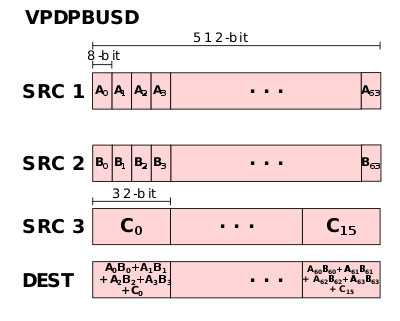
\includegraphics[width=0.5\columnwidth]{Lab-Tex/final/vnni.png}
    \captionof{figure}{Visual explanation of the VPDPBUSD instruction}
    \label{fig:graph_rep}
    \medskip
\endgroup

The supposed tanh implementation is shown below; it undeniably uses fewer instructions.

\begin{lstlisting}
mulss	(%r14), %xmm0
	movss	%xmm0, (%r14)
	movss	4(%rbx), %xmm0          # xmm0 = mem[0],zero,zero,zero
	addss	4(%r15), %xmm0
	addss	%xmm0, %xmm0
	callq	expf
	movss	.LCPI4_0(%rip), %xmm2   # xmm2 = mem[0],zero,zero,zero
	addss	%xmm2, %xmm0
	movss	.LCPI4_1(%rip), %xmm1   # xmm1 = mem[0],zero,zero,zero
	divss	%xmm0, %xmm1
	movaps	%xmm2, %xmm0
	subss	%xmm1, %xmm0
\end{lstlisting}

It was thought that perhaps the LSTM model being used had little to no room to employ the AVX instructions. So, for thorougness, a dense network (which heavily consist of MAC operations) was compiled as well. The new model compiled to use some of the AVX512 instructions, such as ]\cc{vpbroadcastb}. Despite having mutliple locations for MAC instructions, the model still did not use any \cc{vpmadd52huq} instructions.

Although this attempt at compilation could not exploit DLP with the AVX512 instructions, the use of some vector instructions still reduced the total instruction count significantly. Obviously, there were no cases of spillovers, unlike MIPS. 

\section{Conclusion}

As a result of this exploration, a basic understanding of the purpose and design of hardware accelerators was gained. Specifications such as on-board memory or high-bandwidth communication are crucial to producing adequate performance for a machine learning ASIC. Furthermore, the need for a heterogeneous machine learning compiler was also understood. Glow is able to optimize the machine learning model before passing it on for cross-compilation. Exploring the results in different architectures and CPUs was an interesting exercise, showing the limitations and benefits of various architectures. For example, the MIPS CPU's limitation of 32 registers leads to immense communication overhead with memory. \\

Habana, a hardware accelerator startup now acquired by Intel, integrated the Glow compiler as part of their backend. Habana built Goya, a "VLIW CPU based on its own instruction-set architecture, calling it the TPC (Tensor Processor Core)" \cite{habana} (see Figure \ref{fig:habana}). Their chip was able perform quite well in the benchmarks, surpassing NVIDIA's Tesla T4. It is hardware accelerators such as these that benefit from opensource software like Glow, producing superior products while learning and giving back to the ML community. 


 \begingroup
    \centering
    \medskip
    %width=\columnwidth
    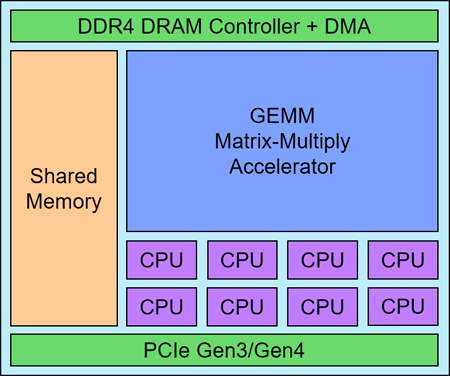
\includegraphics[width=0.5\columnwidth]{Lab-Tex/final/habana.png}
    \captionof{figure}{The Habana chip}
    \label{fig:habana}
    \medskip
\endgroup





%%%%%%%%%%%%%%%%%%%%%%%%%%5
% BIBLIOGRAFIA 
% Estilo de bibliografia ABNT. Se não tiver instalado, mude para plain ou ieeetr

%\bibliographystyle{plain} % Inclua isso se não tiver ABNTEX instalado
% \begin{thebibliography}{refs}
% \bibitem{}
\printbibliography
% \end{thebibliography}
\end{document}